In this section, we describe our proposed approach, \ours, whose high-level diagram and main principles of operation are depicted in Fig.~\ref{fig:nhits_architecture}. Our method extends the \emph{Neural Basis Expansion Analysis} approach (\NBEATS; \citealt{oreshkin2020nbeats}) in several important respects, making it more accurate and computationally efficient, especially in the context of long-horizon forecasting. In essence, our approach uses multi-rate sampling of the input signal and multi-scale synthesis of the forecast, resulting in a hierarchical construction of forecast, greatly reducing computational requirements and improving forecasting accuracy. 
%\NBEATS

Similarly to \NBEATS, \ours\ performs local nonlinear projections onto basis functions across multiple blocks. Each block consists of a \emph{multilayer perceptron} (\MLP), which learns to produce coefficients for the backcast and forecast outputs of its basis. The backcast output is used to clean the inputs of subsequent blocks, while the forecasts are summed to compose the final prediction. The blocks are grouped in stacks, each specialized in learning a different characteristic of the data using a different set of basis functions. The overall network input, $\mathbf{y}_{t-L:t}$, consists of $L$ lags. % of the target time-series $\mathbf{y}$. 

\ours\ is composed of $S$ stacks, $B$ blocks each. Each block contains an \MLP\ predicting forward and backward basis coefficients. The next subsections describe the novel components of our architecture. Note that in the following, we skip the stack index $s$ for brevity.

\subsection{Multi-Rate Signal Sampling}
\label{section:multirate_sampling}
At the input to each block $\ell$, we propose to use a MaxPool layer with kernel size $k_{\ell}$ to help it focus on analyzing components of its input with a specific scale. Larger $k_{\ell}$ will tend to cut more high-frequency/small-time-scale components from the input of the \MLP, forcing the block to focus on analyzing large scale/low frequency content. We call this \emph{multi-rate signal sampling}, referring to the fact that the \MLP\ in each block faces a different effective input signal sampling rate. Intuitively, this helps the blocks with larger pooling kernel size $k_{\ell}$ focus on analyzing large scale components critical for producing consistent long-horizon forecasts. 

% \begin{figure}[ht!]
% \centering
% 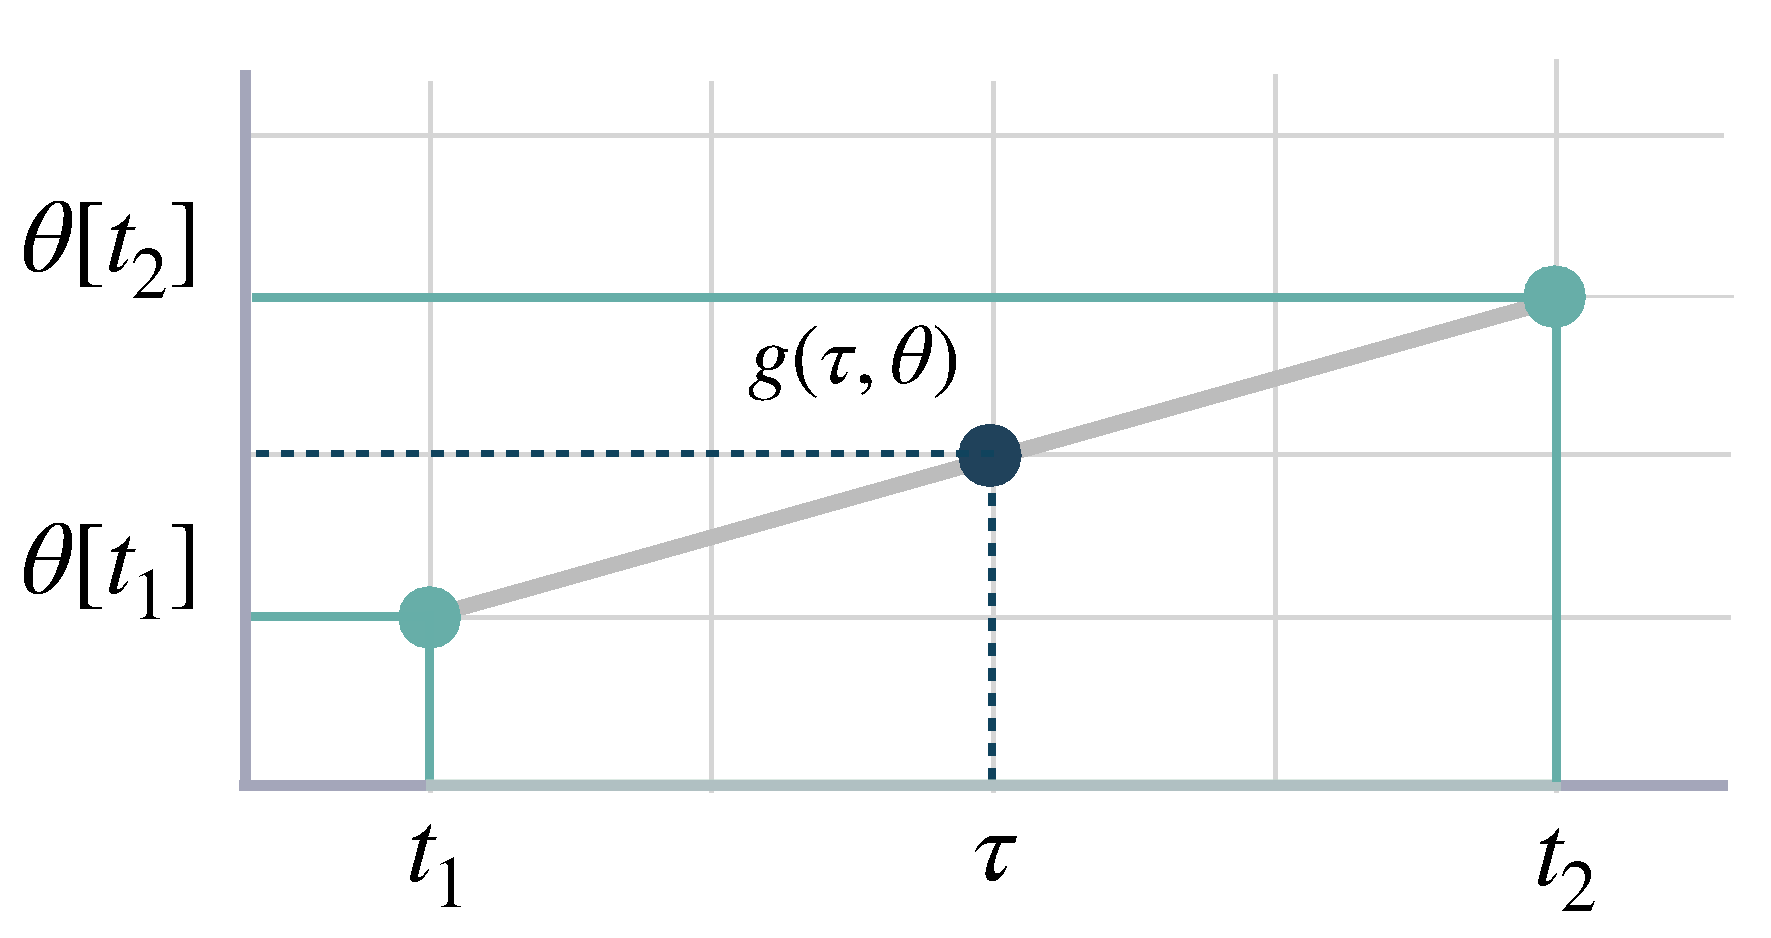
\includegraphics[width=0.65\linewidth]{images/linear_interpolation.pdf}
% \vskip -0.15in
% \caption{The interpolation enhancement to the multi-step forecasting strategy allows \ours\ to reduce the volatility of the predictions through smoothness.} \label{fig:linear_interpolation}
% \end{figure}

Additionally, multi-rate processing reduces the width of the \MLP\ input for most blocks, limiting the memory footprint and the amount of computation as well as  reducing the number of learnable parameters and hence alleviating the effects of overfitting, while maintaining the original receptive field. Given block $\ell$ input $\mathbf{y}_{t-L:t,\ell}$ (the input to the first block $\ell=1$ is the network-wide input, $\mathbf{y}_{t-L:t, 1} \equiv \mathbf{y}_{t-L:t}$), this operation can be formalized as follows:
\begin{equation} \label{equation:nhits_mixed_datasampling}
    \mathbf{y}^{(p)}_{t-L:t, \ell} = \mathbf{MaxPool}\left(\mathbf{y}_{t-L:t, \ell},\; k_{\ell}\right)
\end{equation}

\subsection{Non-Linear Regression}

Following subsampling, block $\ell$ looks at its input and non-linearly regresses forward $\mathbf{\theta}^{f}_{\ell}$ and backward $\mathbf{\theta}^{b}_{\ell}$ interpolation \MLP\ coefficients that learns hidden vector $\mathbf{h}_{\ell} \in \mathbb{R}^{N_{h}}$, which is then linearly projected:
\begin{align} \label{equation:nhits_projections}
\begin{split}
    \mathbf{h}_{\ell}  &= \mathbf{MLP}_{\ell}\left(\mathbf{y}^{(p)}_{t-L:t,\ell}\right) \\
    \btheta^{f}_{\ell} &= \textbf{LINEAR}^{f}\left(\mathbf{h}_{\ell}\right) \\
    \btheta^{b}_{\ell} &= \textbf{LINEAR}^{b}\left(\mathbf{h}_{\ell}\right)
\end{split}
\end{align}
The coefficients are then used to synthesize backcast $\mathbf{\tilde{y}}_{t-L:t,\ell}$ and forecast $\mathbf{\hat{y}}_{t+1:t+H,\ell}$ outputs of the block, via the process described below.

\subsection{Hierarchical Interpolation}
\label{section:hierarchical_interpolation}

In most multi-horizon forecasting models, the cardinality of the neural network prediction equals the dimensionality of horizon, $H$. For example, in \NBEATSi\ $|\btheta^{f}_{\ell}|= H$; in Transformer-based models, decoder attention layer cross-correlates $H$ output embeddings with $L$ encoded input embeddings ($L$ tends to grow with growing $H$). This leads to quick inflation in compute requirements and unnecessary explosion in model expressiveness as horizon $H$ increases.

To combat these issues, we propose to use \emph{temporal interpolation}. We define the dimensionality of the interpolation coefficients in terms of the \emph{expressiveness ratio} $r_{\ell}$ that controls the number of parameters per unit of output time, $|\btheta^{f}_{\ell}|= \lceil r_{\ell} \, H \rceil$. To recover the original sampling rate and predict all $H$ points in the horizon, we use temporal interpolation via the interpolation function $g$:

\begin{align}
\begin{split}
    \hat{y}_{\tau,\ell}   &= g(\tau, \btheta^{f}_{\ell}), \quad \forall \tau \in \{t+1,\dots,t+H\}, \\
    \tilde{y}_{\tau,\ell} &= g(\tau, \btheta^{b}_{\ell}), \quad \forall \tau \in \{t-L,\dots,t\}. 
\end{split}
\end{align}

Interpolation can vary in \emph{smoothness}, $g \in \mathcal{C}^{0}, \mathcal{C}^{1}, \mathcal{C}^{2}$. In Appendix G we explore the nearest neighbor, piece-wise linear and cubic alternatives. For concreteness, the linear interpolator $g \in \mathcal{C}^{1}$, 
along with the time partition $\mathcal{T} = \{t+1, t+1+1/r_{\ell}, \ldots, t+H-1/r_{\ell}, t+H \}$, is defined as

\begin{align}
% \nonumber
\begin{split}
g(\tau, \theta) &= \theta[t_{1}] + \left(\frac{\theta[t_{2}]-\theta[t_{1}]}{t_{2}-t_{1}}\right)(\tau-t_{1}) \\
t_1 &= \arg\min_{t \in \mathcal{T}: t \leq \tau} \tau - t, \quad t_2 = t_1 + 1/r_{\ell}.
\end{split}
\end{align}

\begin{figure}[!t] %t !h
    \centering
    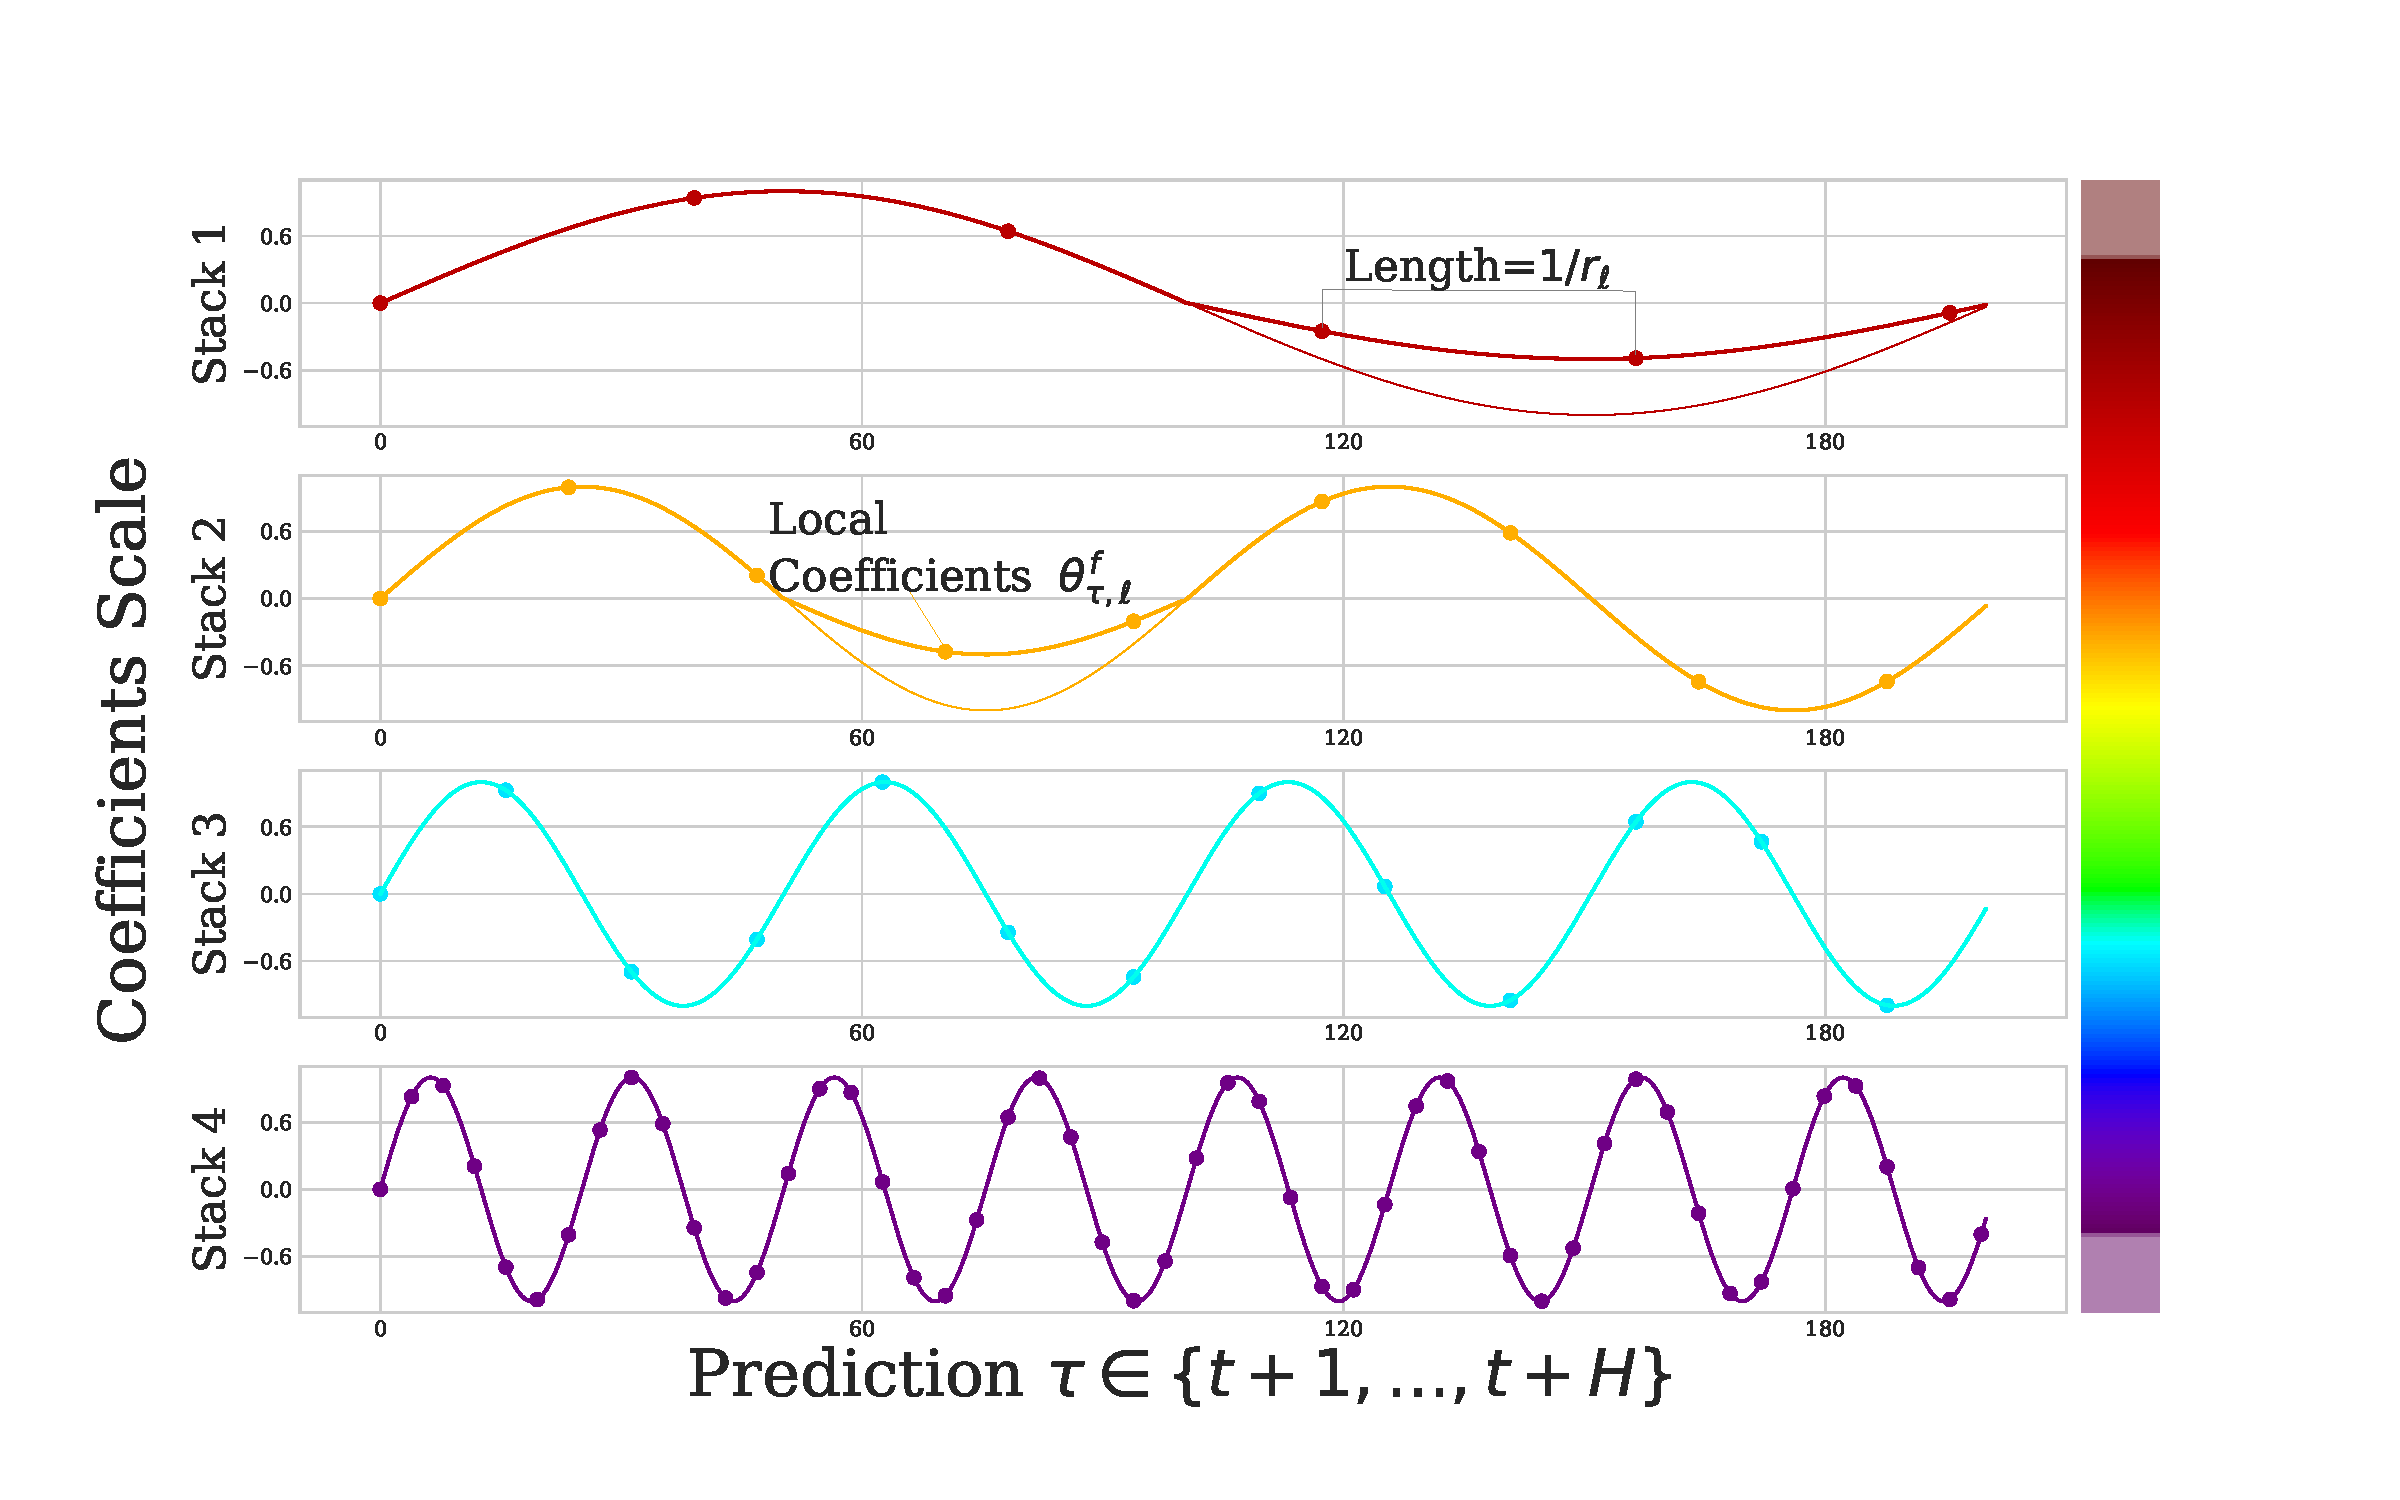
\includegraphics[width=0.95\linewidth]{images/nhits_intuition.pdf}
    \vskip -0.19in
    \caption{\ours\ composes its predictions hierarchically using blocks specialized in different frequencies based on controlled signal projections, through \emph{expressiveness ratios}, and interpolation of each block. The coefficients are locally determined along the horizon, allowing \ours\ to reconstruct non-periodic/stationary signals, beyond constant Fourier transform projections.} \label{fig:nhits_intuition}
\end{figure}

The \emph{hierarchical} interpolation principle is implemented by distributing expressiveness ratios across blocks in a manner synchronized with multi-rate sampling. Blocks closer to the input have smaller $r_{\ell}$ and larger $k_{\ell}$, implying that input blocks generate low-granularity signals via more aggressive interpolation, being also forced to look at more aggressively sub-sampled (and smoothed) signals. The resulting hierarchical forecast $\mathbf{\hat{y}}_{t+1:t+H}$ is assembled by summing the outputs of all blocks, essentially composing it out of interpolations at different time-scale hierarchy levels.

Since each block specializes on its own scale of input and output signal, this induces a clearly structured hierarchy of interpolation granularity, the intuition conveyed in Fig.~\ref{fig:motivation} and \ref{fig:nhits_intuition}. We propose to use \emph{exponentially increasing expressiveness ratios} to handle a wide range of frequency bands while controlling the number of parameters. Alternatively, each stack can specialize in modeling a different known cycle of the time-series (weekly, daily etc.) using a matching $r_{\ell}$ (see Table A.3). Finally, the backcast residual formed at previous hierarchy scale is subtracted from the input of the next hierarchy level to amplify the focus of the next level block on signals outside of the band that has already been handled by the previous hierarchy members.
\begin{equation}
\begin{split}
\mathbf{\hat{y}}_{t+1:t+H} &= \sum^{L}_{l=1} \hat{\mathbf{y}}_{t+1:t+H,\ell} \nonumber \\ \mathbf{y}_{t-L:t,\ell+1} &= \mathbf{y}_{t-L:t,\ell}-\mathbf{\tilde{y}}_{t-L:t,\ell}   %\nonumber
\end{split}
\end{equation}

Hierarchical interpolation has advantageous theoretical guarantees. We show in Appendix A, that it can approximate infinitely/dense horizons. As long as the interpolating function $g$ is characterized by projections to informed multi-resolution functions $V_{w}$, and the forecast relationships are smooth. \\

\textbf{Neural Basis Approximation Theorem.} Let a forecast mapping be $\mathcal{Y}( \cdot \;|\; \ylag ): [0, 1]^L \rightarrow \mathcal{F}$, where the forecast functions $\mathcal{F}=\{\mathcal{Y}(\tau): [0,1] \to \mathbb{R}\}=\mathcal{L}^{2}([0,1])$ representing a infinite/dense horizon, are square integrable. If the multi-resolution functions $V_{w}=\{\phi_{w,h}(\tau) = \phi(2^{w}(\tau-h)) \;|\; w \in {\mathbb{Z}}, h\in2^{-w}\times[0,\dots,2^{w}]\}$ can arbitrarily approximate $\mathcal{L}^{2}([0,1])$. And the projection $\mathrm{Proj}_{V_{w}}(\mathcal{Y}(\tau))$ varies smoothly on $\ylag$. Then the forecast mapping $\mathcal{Y}(\cdot \;|\; \ylag)$ can be arbitrarily approximated by a neural basis expansion learning a finite number of  multi-resolution coefficients $\hat{\theta}_{w,h}$. That is $\forall \epsilon>0$,

\begin{equation}
    \int |\mathcal{Y}(\tau \;|\; \ylag) -\sum_{w,h} \hat{\theta}_{w,h}(\ylag) \phi_{w,h}(\tau) | d\tau \leq \epsilon
\end{equation}

Examples of multi-resolution functions $V_{w}=\{\phi_{w,h}(\tau) = \phi(2^{w}(\tau-h)) \;|\; w \in {\mathbb{Z}}, h\in2^{-w}\times[0,\dots,2^{w}]\}$ include piece-wise constants, piece-wise linear functions and splines with arbitrary approximation capabilities.
